\documentclass[12pt]{article}
\usepackage[utf8]{inputenc}
\usepackage{tikz,egplot}
\usepackage[margin=0.8in]{geometry}
\usepackage{graphicx,ctable}
\usepackage{longtable}
\usepackage{hyperref,xcolor}
\hypersetup{colorlinks=false, linkbordercolor=red,pdfborderstyle={/S/U/W 1}}
\usepackage[para]{threeparttable}
\usepackage{tgpagella}
\usepackage[utf8]{inputenc}
\usepackage{natbib}
\usepackage{caption}
\usepackage{subcaption}
\usepackage{enumitem}
\usepackage[T1]{fontenc}
\setlength{\parindent}{0em}
\usepackage{forest}
\usepackage{booktabs,array,tabularx}
\usepackage{hyperref}
\newcommand{\tab}{\hspace*{3em}}
\hypersetup{
colorlinks = true,
urlcolor = blue,
}
\usepackage{setspace,amsfonts,amssymb,url,booktabs,tabularx,amsmath,amsthm,enumerate}

\title{DNWR and the China Shock}
\date{January 2023}

\begin{document}

\maketitle

\section*{General Information}

\begin{itemize}
    \item We extend the ADH 2013 main regression specification in the following way:
\begin{equation}
    \Delta U_{i,t+h} = \gamma_t + \beta_{1,h} \Delta IPW_{i,\tau} + \beta_{2,h} Rigidity_{i,\tau} \times \Delta IPW_{i,\tau} + \beta_3 Rigidity_{i,\tau} +  X_{i,t}'\beta_4 + \varepsilon_{i,t+h}.\label{eq:ADHreg}
\end{equation}
Similarly to ADH 2021, $\Delta U_{i,t+h}$ is the change in the unemployment per population ratio in CZ $i$ between the initial year $t$ and later year $t + h$ for $h = 1, 
\dots, T$, such that we estimate separate regressions for each time difference between 2000–2006 and 2000–2020. In each regression, we include the 1990-2000 period, as in ADH 2013. The term $\Delta IPW_{i,\tau}$ is the same measure of trade exposure to China used in ADH 2013. We keep it fixed for 1990-2000 and 2000-2007 regardless of $h$ (analogously to ADH 2021). Finally, the variable $Rigidity_{i,\tau}$ stands for a proxy for DNWR. We use several proxies, as discussed below. 
\item We instrument $IPW_{i,\tau}$ with $IPW_{oi,\tau}$, which is constructed using data on contemporaneous industry-level growth of Chinese exports to other high-income markets. This is the same instrument as in ADH 2013. We instrument $Rigidity_{i,\tau} \times \Delta IPW_{i,\tau}$ using $Rigidity_{i,\tau} \times IPW_{oi,\tau}$.
\item We consider the following proxies for $Rigidity_{i,\tau}$:
\begin{itemize}
    \item \ref{sec:r2w}. \textbf{Right-to-work.} Right-to-work laws provide employees the choice not to be a member or to financially support a labor union. Therefore, states with right-to-work laws weakened the role of collective bargaining organizations. The referees expect states with right-to-work laws to see more flexible wages (i.e., less DNWR).  Our first measure of rigidity (state-level) is a dummy variable = 1 if the state has the law by 1990 or 2000. Right-to-work laws by  state were taken from \href{https://nrtwc.org/facts/state-right-to-work-timeline-2016/}{here}. The dta file \textit{right2work.dta} contains the years of implementation by state. 
    \item \ref{sec:negtotal_yjj}. \textbf{Share of negative wage changes to total wage changes (including no-changes) following Yoon Joo Jo (2022).} This uses year-over-year wage changes from CPS data. A higher share implies more wage flexibility. We use a continuous measure but also split states in above/below median.
    \item \ref{sec:negnonzero_yjj}. \textbf{Share of negative wage changes to nonzero wage changes following Yoon Joo Jo (2022).} This uses year-over-year wage changes from CPS data. A higher share implies more wage flexibility. We use a continuous measure but also split states in above/below median.
 
\end{itemize}


    \item  Rigidity measures \ref{sec:negtotal_yjj} and \ref{sec:negnonzero_yjj} were created with data provided by Yoon Joo Jo from her paper ``Establishing downward nominal wage rigidity through cyclical changes in the wage distribution'', 2022 for the 2000 start of period. The file name is \textit{Jo\_state\_level\_dnwr.dta}, with a sample size of 68,312 wage change observations for between 2007 and 2000. For the 1990 start of period, the IPUMS-CPS data was used, with a sample size of 102,034 observations between 1987-1990. 
    \item Each page below presents a Figure with four panels and a table with eight columns. The figure panels show results from 2006 to 2020. For each figure, graph (a) regression specification corresponds to column (3) of the respective table. Graph (b) corresponds to column (6). 
    \item Tables contain coefficients of three specifications at both CZ level and state level. These regressions use the 1990-2000 and 2000-2007 changes in labor market outcomes, as in ADH (2013). Column (1) of each table shows the results of ADH (2013) in their Table 5, Panel B, and Column 3 on unemployment.

\end{itemize}


\newpage
\section{Right-to-work}\label{sec:r2w}
Right-to-work laws by state are implemented using a dummy variable = 1 if the state has the law by 1990 or 2000. Right-to-work laws by state were taken from \href{https://nrtwc.org/facts/state-right-to-work-timeline-2016/}{here}. The dta file \textit{right2work.dta} contains the years of implementation by state. The referees expect states with right-to-work laws to see more flexible wages (i.e., less DNWR).

\begin{figure}[h]\caption{Right-to-work 2006-2020}
     \centering
     \begin{subfigure}[b]{0.45\textwidth}
         \centering
         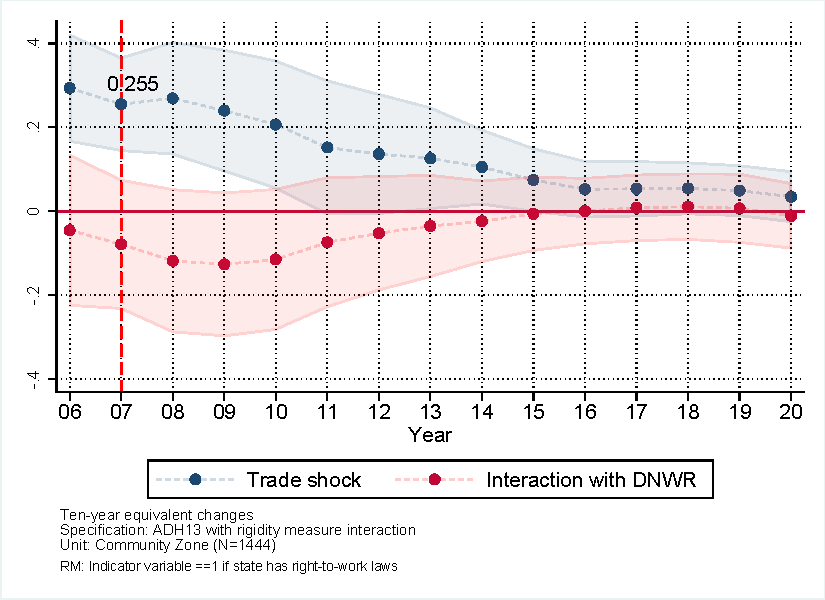
\includegraphics[width=\textwidth]{results/figures/r2w_czs.pdf}
          \caption{CZ-level regression}
     \end{subfigure}
     \hfill
     \begin{subfigure}[b]{0.45\textwidth}
         \centering
         \includegraphics[width=\textwidth]{results/figures/r2w_state.pdf}
         \caption{State-level regression}
     \end{subfigure}
        
\end{figure}
\setstretch{1.0}{\begin{footnotesize} \vspace{-10pt} \textit{Notes:} The figure plots two-stage least squares coefficient estimates for $\beta_{1,h}$ (in blue) and $\beta_{2,h}$ (in red) in equation \eqref{eq:ADHreg} and 95 percent confidence intervals for these estimates. Panels (a) and (b) run the regression at the CZ and state-level, respectively.\end{footnotesize}}


\begin{table}[htbp] \caption{Employment effects of exposure to China shock: r2w}
\centering
\def\sym#1{\ifmmode^{#1}\else\(^{#1}\)\fi}
\large
\resizebox{\textwidth}{!}{%)
\begin{tabular}{l*{8}{c}}
\toprule
                              &\multicolumn{4}{c}{Commuting Zone}                                 &\multicolumn{4}{c}{State}                                          \\\cmidrule(lr){2-5}\cmidrule(lr){6-9}
                              &\multicolumn{1}{c}{(1)}         &\multicolumn{1}{c}{(2)}         &\multicolumn{1}{c}{(3)}         &\multicolumn{1}{c}{(4)}         &\multicolumn{1}{c}{(5)}         &\multicolumn{1}{c}{(6)}         &\multicolumn{1}{c}{(7)}         &\multicolumn{1}{c}{(8)}         \\
                              &    ADH         &Exp/Rig OLS         &Rigidity OLS         &Rigidity IV         &    ADH         &Exp/Rig OLS         &Rigidity OLS         &Rigidity IV         \\
\midrule
Exposure to China             &  0.221\sym{***}&  0.054         &  0.320\sym{***}&  0.255\sym{***}&  0.518\sym{***}&  0.211         &  0.775\sym{***}&  0.703\sym{***}\\
                              &(0.058)         &(0.033)         &(0.073)         &(0.057)         &(0.190)         &(0.185)         &(0.255)         &(0.237)         \\
Exposure interac.             &                & -0.019         & -0.233\sym{***}& -0.079         &                & -0.127         & -0.454\sym{**} & -0.316\sym{*}  \\
                              &                &(0.049)         &(0.071)         &(0.079)         &                &(0.162)         &(0.194)         &(0.181)         \\
\midrule
Observations                  &   1444         &   1444         &   1444         &   1444         &     96         &     96         &     96         &     96         \\
\bottomrule
\end{tabular}%
}
\end{table}

\setstretch{1.0}{\begin{footnotesize} \vspace{-10pt} \textit{Notes:} The table shows regression coefficients for $\beta_{1,h}$ (Exposure to China) and $\beta_{2,h}$ (Exposure interac) in equation \eqref{eq:ADHreg}. Columns (1)-(4) focus on CZ-level regressions, and Columns (5)-(8) on State-level regressions. Column (1) corresponds to the ADH 2013 results and column (5) is its analogous state-level counterpart. Columns (2) and (6) use OLS. Columns (3) and (7) instrument exposure to China but not the interaction term. Columns (4) and (8) use both instruments. As in ADH 2013, the regression covers the period from 1990-2000 and 2000-2007 with stacked first differences.\end{footnotesize}}
%%%%%%%%%%%%%%%%%%%%%%%%%%%%%%%%%%%%%%%%%%%%%%%%%%%%%
\newpage


\section{Share of negative wage changes to total wage changes: CPS} \label{sec:negtotal_yjj}
Total downward wage adjustments share of total wage changes. Year-over-year changes. A higher share of negative wage changes indicates lower downward nominal wage rigidity.

\subsection{Share of negative wage changes of total wage changes (indicator = 1 if above median): CPS}

\begin{figure}[h]\caption{Negative share of total wage changes (above median dummy) 2006-2020}
     \centering
     \begin{subfigure}[b]{0.45\textwidth}
         \centering
         \includegraphics[width=\textwidth]{results/figures/dnwr_yjj_dmy1_czs.pdf}
         \caption{CZ-level regression}
     \end{subfigure}
     \hfill
     \begin{subfigure}[b]{0.45\textwidth}
         \centering
         \includegraphics[width=\textwidth]{results/figures/dnwr_yjj_dmy1_state.pdf}
         \caption{State-level regression}
     \end{subfigure}
        
\end{figure}
\setstretch{1.0}{\begin{footnotesize} \vspace{-10pt} \textit{Notes:} The figure plots two-stage least squares coefficient estimates for $\beta_{1,h}$ (in blue) and $\beta_{2,h}$ (in red) in equation \eqref{eq:ADHreg} and 95 percent confidence intervals for these estimates. Panels (a) and (b) run the regression at the CZ and state-level, respectively.\end{footnotesize}}

\begin{table}[htbp] \caption{Employment effects of exposure to China shock: dnwr\_yjj\_dmy1}
\centering
\def\sym#1{\ifmmode^{#1}\else\(^{#1}\)\fi}
\large
\resizebox{\textwidth}{!}{%)
\begin{tabular}{l*{8}{c}}
\toprule
                              &\multicolumn{4}{c}{Commuting Zone}                                 &\multicolumn{4}{c}{State}                                          \\\cmidrule(lr){2-5}\cmidrule(lr){6-9}
                              &\multicolumn{1}{c}{(1)}         &\multicolumn{1}{c}{(2)}         &\multicolumn{1}{c}{(3)}         &\multicolumn{1}{c}{(4)}         &\multicolumn{1}{c}{(5)}         &\multicolumn{1}{c}{(6)}         &\multicolumn{1}{c}{(7)}         &\multicolumn{1}{c}{(8)}         \\
                              &    ADH         &Exp/Rig OLS         &Rigidity OLS         &Rigidity IV         &    ADH         &Exp/Rig OLS         &Rigidity OLS         &Rigidity IV         \\
\midrule
Exposure to China             &  0.221\sym{***}&  0.004         &  0.259         &  0.122         &  0.518\sym{***}&  0.303         &  0.882\sym{***}&  0.811\sym{***}\\
                              &(0.058)         &(0.035)         &(0.186)         &(0.088)         &(0.190)         &(0.188)         &(0.273)         &(0.245)         \\
Exposure interac.             &                & -0.048         & -0.261\sym{*}  & -0.030         &                & -0.234         & -0.568\sym{***}& -0.460\sym{**} \\
                              &                &(0.041)         &(0.152)         &(0.072)         &                &(0.157)         &(0.198)         &(0.179)         \\
\midrule
Observations                  &   1444         &    722         &    722         &    722         &     96         &     96         &     96         &     96         \\
\bottomrule
\end{tabular}%
}
\end{table}

\setstretch{1.0}{\begin{footnotesize} \vspace{-10pt} \textit{Notes:} The table shows regression coefficients for $\beta_{1,h}$ (Exposure to China) and $\beta_{2,h}$ (Exposure interac) in equation \eqref{eq:ADHreg}. Columns (1)-(4) focus on CZ-level regressions, and Columns (5)-(8) on State-level regressions. Column (1) corresponds to the ADH 2013 results and column (5) is its analogous state-level counterpart. Columns (2) and (6) use OLS. Columns (3) and (7) instrument exposure to China but not the interaction term. Columns (4) and (8) use both instruments. As in ADH 2013, the regression covers the period from 1990-2000 and 2000-2007 with stacked first differences.\end{footnotesize}}

\newpage
\subsection{Share of negative wage changes of total wage changes (indicator = 1 if above mean): CPS}

\begin{figure}[h]\caption{Negative share of total wage changes (above mean dummy) 2006-2020}

     \centering
     \begin{subfigure}[b]{0.45\textwidth}
         \centering
         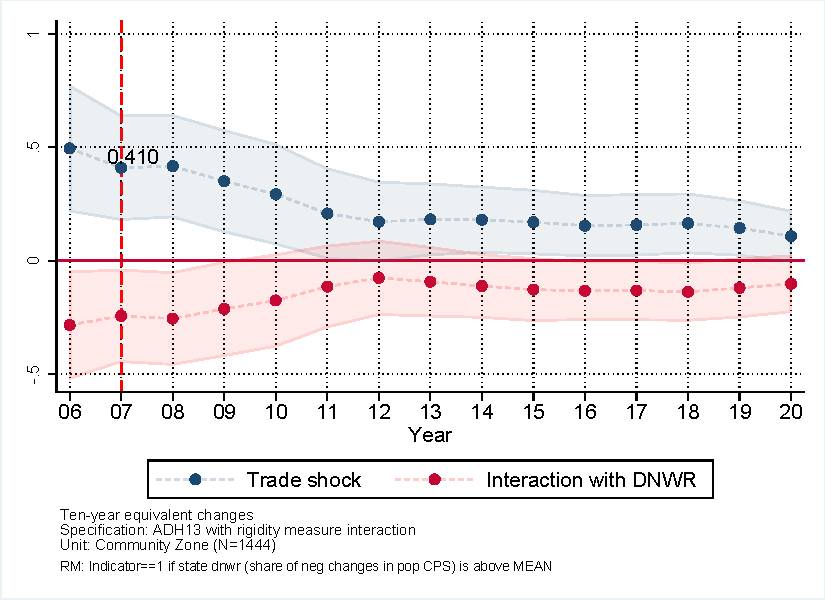
\includegraphics[width=\textwidth]{results/figures/dnwr_yjj_dmy2_czs.pdf}
         \caption{CZ-level regression}
     \end{subfigure}
     \hfill
     \begin{subfigure}[b]{0.45\textwidth}
         \centering
         \includegraphics[width=\textwidth]{results/figures/dnwr_yjj_dmy2_state.pdf}
         \caption{State-level regression}
     \end{subfigure}
        
\end{figure}
\setstretch{1.0}{\begin{footnotesize} \vspace{-10pt} \textit{Notes:} The figure plots two-stage least squares coefficient estimates for $\beta_{1,h}$ (in blue) and $\beta_{2,h}$ (in red) in equation \eqref{eq:ADHreg} and 95 percent confidence intervals for these estimates. Panels (a) and (b) run the regression at the CZ and state-level, respectively.\end{footnotesize}}

\begin{table}[htbp] \caption{Employment effects of exposure to China shock: dnwr\_yjj\_dmy2}
\centering
\def\sym#1{\ifmmode^{#1}\else\(^{#1}\)\fi}
\large
\resizebox{\textwidth}{!}{%)
\begin{tabular}{l*{8}{c}}
\toprule
                              &\multicolumn{4}{c}{Commuting Zone}                                 &\multicolumn{4}{c}{State}                                          \\\cmidrule(lr){2-5}\cmidrule(lr){6-9}
                              &\multicolumn{1}{c}{(1)}         &\multicolumn{1}{c}{(2)}         &\multicolumn{1}{c}{(3)}         &\multicolumn{1}{c}{(4)}         &\multicolumn{1}{c}{(5)}         &\multicolumn{1}{c}{(6)}         &\multicolumn{1}{c}{(7)}         &\multicolumn{1}{c}{(8)}         \\
                              &    ADH         &Exp/Rig OLS         &Rigidity OLS         &Rigidity IV         &    ADH         &Exp/Rig OLS         &Rigidity OLS         &Rigidity IV         \\
\midrule
Exposure to China             &  0.221\sym{***}&  0.098\sym{*}  &  0.631\sym{***}&  0.410\sym{***}&  0.518\sym{***}&  0.302         &  0.897\sym{***}&  0.820\sym{***}\\
                              &(0.058)         &(0.053)         &(0.215)         &(0.119)         &(0.190)         &(0.189)         &(0.277)         &(0.247)         \\
Exposure interac.             &                & -0.082         & -0.529\sym{***}& -0.243\sym{**} &                & -0.236         & -0.585\sym{***}& -0.469\sym{**} \\
                              &                &(0.067)         &(0.187)         &(0.105)         &                &(0.160)         &(0.203)         &(0.183)         \\
\midrule
Observations                  &   1444         &   1444         &   1444         &   1444         &     96         &     96         &     96         &     96         \\
\bottomrule
\end{tabular}%
}
\end{table}

\setstretch{1.0}{\begin{footnotesize} \vspace{-10pt} \textit{Notes:} The table shows regression coefficients for $\beta_{1,h}$ (Exposure to China) and $\beta_{2,h}$ (Exposure interac) in equation \eqref{eq:ADHreg}. Columns (1)-(4) focus on CZ-level regressions, and Columns (5)-(8) on State-level regressions. Column (1) corresponds to the ADH 2013 results and column (5) is its analogous state-level counterpart. Columns (2) and (6) use OLS. Columns (3) and (7) instrument exposure to China but not the interaction term. Columns (4) and (8) use both instruments. As in ADH 2013, the regression covers the period from 1990-2000 and 2000-2007 with stacked first differences.\end{footnotesize}}

\newpage

\section{Share of negative wage changes of nonzero variations: CPS} \label{sec:negnonzero_yjj}
Total downward wage adjustments share of nonzero wage changes. A higher share of negative wage changes relative to the total nonzero wage changes indicates a lower downward nominal wage rigidity. Year-over-year wage changes.

\subsection{Share of negative wage changes of nonzero variations (indicator = 1 if above median): CPS}

\begin{figure}[h]\caption{Share of negative wage changes of nonzero variations (above median dummy) 2006-2020}
     \centering
     \begin{subfigure}[b]{0.45\textwidth}
         \centering
         \includegraphics[width=\textwidth]{results/figures/dnwr_nonzero_yjj_dmy1_czs.pdf}
         \caption{CZ-level regression}
     \end{subfigure}
     \hfill
     \begin{subfigure}[b]{0.45\textwidth}
         \centering
         \includegraphics[width=\textwidth]{results/figures/dnwr_nonzero_yjj_dmy1_state.pdf}
         \caption{State-level regression}
     \end{subfigure}
        
\end{figure}
\setstretch{1.0}{\begin{footnotesize} \vspace{-10pt} \textit{Notes:} The figure plots two-stage least squares coefficient estimates for $\beta_{1,h}$ (in blue) and $\beta_{2,h}$ (in red) in equation \eqref{eq:ADHreg} and 95 percent confidence intervals for these estimates. Panels (a) and (b) run the regression at the CZ and state-level, respectively.\end{footnotesize}}

\begin{table}[htbp] \caption{Employment effects of exposure to China shock: dnwr\_nonzero\_yjj\_dmy1}
\centering
\def\sym#1{\ifmmode^{#1}\else\(^{#1}\)\fi}
\large
\resizebox{\textwidth}{!}{%)
\begin{tabular}{l*{8}{c}}
\toprule
                              &\multicolumn{4}{c}{Commuting Zone}                                 &\multicolumn{4}{c}{State}                                          \\\cmidrule(lr){2-5}\cmidrule(lr){6-9}
                              &\multicolumn{1}{c}{(1)}         &\multicolumn{1}{c}{(2)}         &\multicolumn{1}{c}{(3)}         &\multicolumn{1}{c}{(4)}         &\multicolumn{1}{c}{(5)}         &\multicolumn{1}{c}{(6)}         &\multicolumn{1}{c}{(7)}         &\multicolumn{1}{c}{(8)}         \\
                              &    ADH         &Exp/Rig OLS         &Rigidity OLS         &Rigidity IV         &    ADH         &Exp/Rig OLS         &Rigidity OLS         &Rigidity IV         \\
\midrule
Exposure to China             &  0.221\sym{***}&  0.001         &  0.253         &  0.112         &  0.518\sym{***}&  0.296         &  0.865\sym{***}&  0.788\sym{***}\\
                              &(0.058)         &(0.033)         &(0.180)         &(0.081)         &(0.190)         &(0.186)         &(0.269)         &(0.242)         \\
Exposure interac.             &                & -0.046         & -0.256\sym{*}  & -0.016         &                & -0.218         & -0.543\sym{***}& -0.424\sym{**} \\
                              &                &(0.041)         &(0.149)         &(0.072)         &                &(0.157)         &(0.195)         &(0.177)         \\
\midrule
Observations                  &   1444         &    722         &    722         &    722         &     96         &     96         &     96         &     96         \\
\bottomrule
\end{tabular}%
}
\end{table}

\setstretch{1.0}{\begin{footnotesize} \vspace{-10pt} \textit{Notes:} The table shows regression coefficients for $\beta_{1,h}$ (Exposure to China) and $\beta_{2,h}$ (Exposure interac) in equation \eqref{eq:ADHreg}. Columns (1)-(4) focus on CZ-level regressions, and Columns (5)-(8) on State-level regressions. Column (1) corresponds to the ADH 2013 results and column (5) is its analogous state-level counterpart. Columns (2) and (6) use OLS. Columns (3) and (7) instrument exposure to China but not the interaction term. Columns (4) and (8) use both instruments. As in ADH 2013, the regressions cover the period from 1990-2000 and 2000-2007 with stacked first differences, with a constant and a dummy for the 2000-2007 period.\end{footnotesize}}

\newpage
\subsection{Share of negative wage changes of nonzero wage changes (indicator = 1 if above mean): CPS}

\begin{figure}[h]\caption{Share of negative wage changes of nonzero variations (above mean dummy) 2006-2020}
     \centering
     \begin{subfigure}[b]{0.45\textwidth}
         \centering
         \includegraphics[width=\textwidth]{results/figures/dnwr_nonzero_yjj_dmy2_czs.pdf}
         \caption{CZ-level regression}
     \end{subfigure}
     \hfill
     \begin{subfigure}[b]{0.45\textwidth}
         \centering
         \includegraphics[width=\textwidth]{results/figures/dnwr_nonzero_yjj_dmy2_state.pdf}
         \caption{State-level regression}
     \end{subfigure}
        
\end{figure}
\setstretch{1.0}{\begin{footnotesize} \vspace{-10pt} \textit{Notes:} The figure plots two-stage least squares coefficient estimates for $\beta_{1,h}$ (in blue) and $\beta_{2,h}$ (in red) in equation \eqref{eq:ADHreg} and 95 percent confidence intervals for these estimates. Panels (a) and (b) run the regression at the CZ and state-level, respectively.\end{footnotesize}}

\begin{table}[htbp] \caption{Employment effects of exposure to China shock: dnwr\_nonzero\_yjj\_dmy2}
\centering
\def\sym#1{\ifmmode^{#1}\else\(^{#1}\)\fi}
\large
\resizebox{\textwidth}{!}{%)
\begin{tabular}{l*{8}{c}}
\toprule
                              &\multicolumn{4}{c}{Commuting Zone}                                 &\multicolumn{4}{c}{State}                                          \\\cmidrule(lr){2-5}\cmidrule(lr){6-9}
                              &\multicolumn{1}{c}{(1)}         &\multicolumn{1}{c}{(2)}         &\multicolumn{1}{c}{(3)}         &\multicolumn{1}{c}{(4)}         &\multicolumn{1}{c}{(5)}         &\multicolumn{1}{c}{(6)}         &\multicolumn{1}{c}{(7)}         &\multicolumn{1}{c}{(8)}         \\
                              &    ADH         &Exp/Rig OLS         &Rigidity OLS         &Rigidity IV         &    ADH         &Exp/Rig OLS         &Rigidity OLS         &Rigidity IV         \\
\midrule
Exposure to China             &  0.221\sym{***}&  0.094\sym{*}  &  0.613\sym{***}&  0.396\sym{***}&  0.518\sym{***}&  0.299         &  0.894\sym{***}&  0.812\sym{***}\\
                              &(0.058)         &(0.051)         &(0.206)         &(0.117)         &(0.190)         &(0.189)         &(0.275)         &(0.247)         \\
Exposure interac.             &                & -0.075         & -0.506\sym{***}& -0.223\sym{**} &                & -0.219         & -0.561\sym{***}& -0.438\sym{**} \\
                              &                &(0.066)         &(0.178)         &(0.103)         &                &(0.159)         &(0.200)         &(0.180)         \\
\midrule
Observations                  &   1444         &   1444         &   1444         &   1444         &     96         &     96         &     96         &     96         \\
\bottomrule
\end{tabular}%
}
\end{table}

\setstretch{1.0}{\begin{footnotesize} \vspace{-10pt} \textit{Notes:} The table shows regression coefficients for $\beta_{1,h}$ (Exposure to China) and $\beta_{2,h}$ (Exposure interac) in equation \eqref{eq:ADHreg}. Columns (1)-(4) focus on CZ-level regressions, and Columns (5)-(8) on State-level regressions. Column (1) corresponds to the ADH 2013 results and column (5) is its analogous state-level counterpart. Columns (2) and (6) use OLS. Columns (3) and (7) instrument exposure to China but not the interaction term. Columns (4) and (8) use both instruments. As in ADH 2013, the regression covers the period from 1990-2000 and 2000-2007 with stacked first differences.\end{footnotesize}}
\newpage

\end{document}